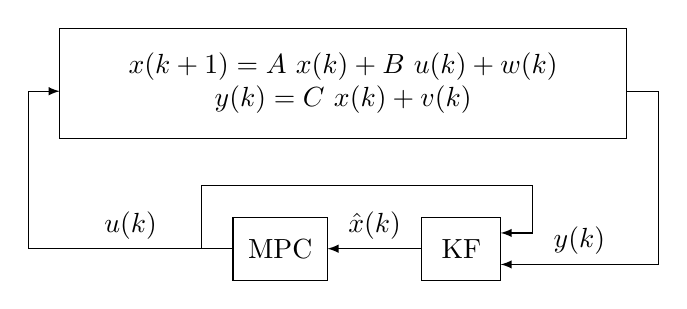
\begin{tikzpicture}
\draw  (-2.8,3.6) rectangle (4.4,2.2) node[midway,align=center] {$x(k+1)=A~x(k)+B~u(k)+w(k)$\\ $y(k)=C~x(k)+v(k)$ };
\draw [-latex] (4.4,2.8) --  (4.8,2.8)  -- (4.8,0.6) -- (2.8,0.6) node[midway,above]{$y(k)$};
\draw  (1.8,1.2) rectangle (2.8,0.4) node[midway,align=center] {KF};
\draw [-latex] (1.8,0.8)  -- (0.6,0.8) node[above,midway]{$\hat{x}(k)$};
\draw (-0.6,1.2) rectangle (0.6,0.4) node[midway,align=center] {MPC};
\draw [-latex] (-0.6,0.8)  -- node[above]{$u(k)$} (-3.2,0.8)  -- (-3.2,2.8) -- (-2.8,2.8);
\draw [-latex] (-1,0.8)  -- (-1,1.6) -- (3.2,1.6) -- (3.2,1) -- (2.8,1);
\end{tikzpicture}